\chapter{Dasar Teori}
\label{chap:Dasar Teori}

\section{jsoup}
\label{sec:jsoup}

\textit{Web Scraping} adalah teknik yang digunakan untuk mendapatkan informasi dari sebuah \textit{website}
secara otomatis. Dalam Java, \textit{web scraping} dapat diimplementasikan menggunakan \textit{library} jsoup \cite{jsoup}. API yang disediakan oleh jsoup dapat digunakan untuk menyeleksi dan memanipulasi data. Elemen HTML akan di-\textit{parse} ke dalam bentuk \textit{Document Object Model} (DOM) yang direpresentasikan dalam kelas Document. Dalam menyeleksi data, jsoup memanfaatkan CSS \textit{Selector} untuk mendapatkan elemen HTML yang diinginkan dari objek Document hasil \textit{parsing} HTML. Hasil proses seleksi akan ditampung ke dalam objek bertipe Element yang merepresentasikan elemen pada HTML. Kemudian elemen yang diperoleh dapat dimanipulasi sesuai kebutuhan.

\section{Chrome DevTools}
\label{sec:devtools}

Chrome Developer Tools (DevTools) \cite{devtools} adalah perangkat \textit{debugging} yang dimiliki Google Chrome. \textit{Developer tools} sendiri berfungsi untuk melakukan \textit{debugging} terhadap suatu \textit{website}. DevTools dapat melakukan debugging terhadap website yang dikunjunginya.

Fitur-fitur yang dimiliki DevTools antara lain:
\begin{enumerate}
	\item \textit{Elements}, memeriksa dan mengubah elemen HTML dan \textit{style} dari suatu \textit{website}.
	\item \textit{Console}, mendapatkan informasi pengembangan dan berinteraksi dengan dokumen.
	\item \textit{Sources}, melakukan \textit{debugging} pada JavaScript dengan menentukan \textit{breakpoint}.
	\item \textit{Network}, memantau kinerja jaringan pada \textit{website} secara \textit{real-time}.
	\item \textit{Audits}, menganalisa halaman yang dimuat.
	\item \textit{Timeline}, menampilkan alur waktu saat memuat halaman.
	\item \textit{Profiles}, menggambarkan waktu eksekusi dan penggunaan memori saat memuat halaman.
	\item \textit{Resources}, memeriksa sumber daya halaman yang dapat berupa basis data, \textit{cookies}, dan \textit{cache}.
\end{enumerate}

\begin{figure}
	\centering
	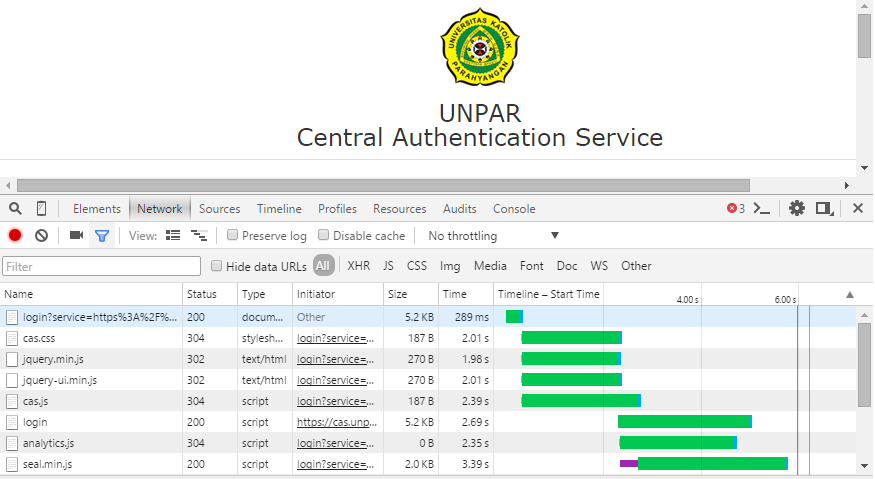
\includegraphics[scale=0.5]{Gambar/chrome-devtools}
	\caption{Chrome DevTools} 
	\label{fig:chrome_devtools}
\end{figure}

\section{Play Framework}
\label{sec:play}

Play Framework \cite{Leroux:2014} merupakan sebuah web framework berbasis Java dan Scala. Play juga menggunakan \textit{design pattern} Model-View-Controller (MVC) di mana \textit{model} dan \textit{controller} menggunakan Java sedangkan \textit{view} menggunakan Scala dan HTML. 
